\documentclass{beamer}
\usepackage[utf8]{inputenc}

\usetheme{Madrid}
\usecolortheme{default}
\usepackage{amsmath,amssymb,amsfonts,amsthm}
\usepackage{txfonts}
\usepackage{tkz-euclide}
\usepackage{listings}
\usepackage{adjustbox}
\usepackage{array}
\usepackage{tabularx}
\usepackage{gvv}
\usepackage{lmodern}
\usepackage{circuitikz}
\usepackage{tikz}
\usepackage{graphicx}

\setbeamertemplate{page number in head/foot}[totalframenumber]

\usepackage{tcolorbox}
\tcbuselibrary{minted,breakable,xparse,skins}



\definecolor{bg}{gray}{0.95}
\DeclareTCBListing{mintedbox}{O{}m!O{}}{%
  breakable=true,
  listing engine=minted,
  listing only,
  minted language=#2,
  minted style=default,
  minted options={%
    linenos,
    gobble=0,
    breaklines=true,
    breakafter=,,
    fontsize=\small,
    numbersep=8pt,
    #1},
  boxsep=0pt,
  left skip=0pt,
  right skip=0pt,
  left=25pt,
  right=0pt,
  top=3pt,
  bottom=3pt,
  arc=5pt,
  leftrule=0pt,
  rightrule=0pt,
  bottomrule=2pt,
  toprule=2pt,
  colback=bg,
  colframe=orange!70,
  enhanced,
  overlay={%
    \begin{tcbclipinterior}
    \fill[orange!20!white] (frame.south west) rectangle ([xshift=20pt]frame.north west);
    \end{tcbclipinterior}},
  #3,
}
\lstset{
    language=C,
    basicstyle=\ttfamily\small,
    keywordstyle=\color{blue},
    stringstyle=\color{orange},
    commentstyle=\color{green!60!black},
    numbers=left,
    numberstyle=\tiny\color{gray},
    breaklines=true,
    showstringspaces=false,
}
%------------------------------------------------------------
%This block of code defines the information to appear in the
%Title page
\title %optional
{1.5.1}
\date{August 27, 2025}

\author 
{Shreyas Goud Burra - EE25BTECH11051}


\begin{document}

\frame{\titlepage}
\begin{frame}{Question}
    Find the ratio in which the Y axis divides the line segment joining the points (6, -4)
and (-2, -7). Also find the point of intersection.

\end{frame}
\begin{frame}{Given Information}
    Assume the two points to be position vectors $\textbf{A} = \myvec{6 \\ -4}$ and $\textbf{B} = \myvec{-2 \\ -7}$
\end{frame}

\begin{frame}{Formula}
To find the ratio in which the Y axis divides the line segment. We can use the section formula\\
    \begin{align}
        \textbf{C} = \brak{\frac{\frac{m}{n}A+B}{\frac{m}{n}+1}}
        \label{0.1}
    \end{align}
Where \textbf{C} is the point on the Y axis that intersects given line segment
\end{frame}
\begin{frame}{Solution}
    Here we can assume some constant $k=\frac{m}{n}$. This gives us

\begin{align}
    \textbf{C} = \brak{\frac{kA+B}{k+1}}
    \label{0.2}
\end{align}
\end{frame}
\begin{frame}{Continuation}
    We can write \textbf{C} as 
    
    \begin{align}
        \mathbf{C} = \myvec{0 \\ y}
        \label{0.3}
    \end{align}
    Where $y$ is the y coordinate of the point of intersection of the Y axis and the line segment AB.
\end{frame}

\begin{frame}{Continuation}
We know that these three points are collinear, so by using rank method we get. Rank of matrix 
\begin{align}
    \textbf{P} = (\textbf{B}-\textbf{A} \text{ } \textbf{C}-\textbf{A}) = 1 \\
    \implies \text{Rank of } \myvec{-8 & -6 \\ -3 & y+4} = 1
    \label{0.4}
\end{align}
\end{frame}
\begin{frame}{Continuation}
On applying row transformations

$$ R_2 \rightarrow R_2 - \frac{3}{8}R_1$$

\begin{align}
    \textbf{C} = \myvec{-8 & -6 \\ 0 & y+\frac{25}{4}}\\
\end{align}
\end{frame}

\begin{frame}{Continuation}
If rank = 0

\begin{align}
    \implies y+\frac{25}{4} = 0\\
    y = -\frac{25}{4}
\end{align}
\end{frame}

\begin{frame}[fragile]
    \frametitle{Python Code}
    \begin{lstlisting}
import numpy as np
import matplotlib.pyplot as plt
import ctypes

def line_gen_num(A,B,num):
  dim = A.shape[0]
  x_AB = np.zeros((dim,num))
  lam_1 = np.linspace(0,1,num)
  for i in range(num):
    temp1 = A + lam_1[i]*(B-A)
    x_AB[:,i]= temp1.T
  return x_AB

\end{lstlisting}
\end{frame}

\begin{frame}[fragile]
\frametitle{Python Code}
    \begin{lstlisting}

# Define 2D points A and B
A = np.array([6, -4])
B = np.array([-2, -7])

k = 1/3 #ratio

C = ((k*A+B)/(k+1))

# Generate line points
x_AB = line_gen_num(A, B, 20)

# Plotting

\end{lstlisting}
\end{frame}

\begin{frame}[fragile]
\frametitle{Python Code}
    \begin{lstlisting}

plt.grid()
plt.title('1.5.1')
plt.plot(x_AB[0, :], x_AB[1, :], 'r--', label='Line from A to B')  # 'bo-' = blue dots with lines
plt.plot(A[0], A[1], 'go', label='Point A')  # green dot
plt.annotate('(6,-4)', xy=(A[0],A[1]), fontsize=12)
plt.plot(B[0], B[1], 'go', label='Point B')  # red dot
plt.annotate('(-2,-7)', xy=(B[0],B[1]), fontsize=12)
plt.plot(C[0], C[1], 'bo', label='Intersection Point') #intersection point
plt.legend()
\end{lstlisting}
\end{frame}

\begin{frame}[fragile]
\frametitle{Python Code}
    \begin{lstlisting}
plt.xlabel('X-axis')
plt.ylabel('Y-axis')
plt.axis('equal')
plt.savefig('/figs/fig1.png')

plt.show()

    \end{lstlisting}
    
\end{frame}

\begin{frame}{Plot}
    \begin{figure}[H]
    \centering
    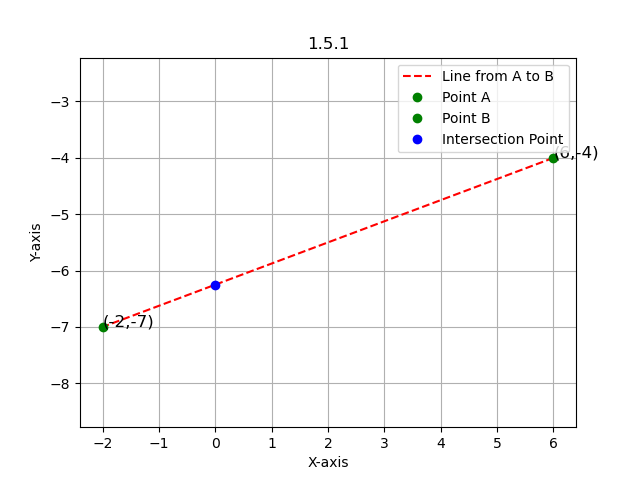
\includegraphics[width=0.6\columnwidth]{figs/fig1.png}
    \caption{Intersection of line segment with Y axis}
    \label{2D Plot}
\end{figure}
\end{frame}
\end{document}